\documentclass[../main.tex]{subfiles}
\begin{document}
\section{Políticas y Control de Acceso}

\begin{examen}
Esta es \textbf{la unidad más evaluada} del segundo parcial: aparece en casi todos los exámenes. Los temas estrella son:
\begin{itemize}[nosep]
  \item \textbf{Diseño de compartimentos} (construir un retículo a partir de un enunciado en lenguaje natural). Confidencialidad (Bell-LaPadula) e integridad (Biba/Clark-Wilson).
  \item Identificar la política dado un retículo, y nombrarla bien (BLP vs Biba).
  \item Resolución de conflictos entre reglas (first-match, best-match, deny-over-allow, grant-all).
  \item Distinguir \textbf{modelo} / \textbf{política} / \textbf{reglas} de seguridad.
  \item Preguntas conceptuales V/F (matriz de acceso, ACL vs Capabilities).
  \item Ejercicios abiertos tipo ``sos el CSO'': elegir objetivo de seguridad, modelo, política y reglas.
\end{itemize}
\end{examen}

%======================================================================
\subsection{Conceptos base}
%======================================================================

\subsubsection{¿Qué es seguridad? Política y estados}

No hay una única definición de seguridad. Igual que en criptografía cada prueba daba una definición distinta de seguridad, al pasar a sistemas dinámicos tampoco hay una definición única. La definición genérica que se usa es:

\begin{definicion}{Sistema seguro}
Si podemos clasificar todos los estados de un sistema en \textbf{seguros} e \textbf{inseguros}, un sistema es seguro mientras sus estados queden dentro de la política de seguridad (mientras transicione solo por estados que consideramos seguros).
\end{definicion}

\begin{definicion}{Política de seguridad}
Es la definición de qué estados de un sistema vamos a considerar seguros versus el resto. En un contexto (aplicación, servicio, empresa) la política define los modos y usos que se consideran seguros.
\end{definicion}

Dos conceptos potentes de esta definición:
\begin{enumerate}[nosep]
  \item Necesitamos poder caracterizar, ``sacando una foto'' del estado actual, si es seguro o no.
  \item Un sistema que pasa a un estado inseguro \textbf{deja de ser seguro, aunque después vuelva} a un estado seguro. Por eso, ante un servidor comprometido, las buenas prácticas dicen reinstalarlo desde cero: es muy difícil volver a un estado de confianza.
\end{enumerate}

\subsubsection{La tríada CIA}

\begin{itemize}[nosep]
  \item \textbf{Confidencialidad}: atañe a la diseminación de información. Hay información accesible a cierto grupo y no a otro.
  \item \textbf{Integridad}: tiene que ver con relaciones de confianza. Garantizar/certificar la calidad de algo (que una transacción ocurre, que los datos son correctos, que el origen es quien dice ser).
  \item \textbf{Disponibilidad}: capacidad de acceder a información o ejecutar una acción en el momento dado. Involucra temporalidad, es dinámica y por eso no se estudia tanto en criptografía (que era estática).
\end{itemize}

\subsubsection{Sujeto, Objeto, Acceso}

\begin{definicion}{Sujeto / Objeto / Acceso}
\textbf{Sujeto}: entidad que ejecuta cosas sobre otras entidades; es el origen de un estímulo. Puede ser persona, servicio, aplicación, servidor.\\
\textbf{Objeto}: destino de esos estímulos. Generalmente recursos: datos, servicios, bases de datos, tablas, programas, archivos.\\
\textbf{Acceso}: las formas que tienen los sujetos de interactuar con el objeto (leer, escribir, borrar, mover, ejecutar\dots).
\end{definicion}

Ejemplo: en Linux los sujetos son usuarios, los objetos son archivos (todo es un archivo) y los accesos son permisos. La tríada se reduce a esta base:
\begin{itemize}[nosep]
  \item \textbf{Confidencialidad}: existen sujetos que \underline{NO pueden acceder} a ciertos objetos.
  \item \textbf{Integridad}: existen objetos que \underline{solo pueden ser modificados} por ciertos sujetos confiables.
  \item \textbf{Disponibilidad}: existen objetos que pueden ser accedidos por ciertos sujetos \underline{cuando lo requieran}.
\end{itemize}

\textbf{Identidad del sujeto}: lo que identifica unívocamente al sujeto dentro del universo de posibles sujetos. Es requisito para la autenticación (ej.\ SID en Windows, UID en \texttt{/etc/passwd}).

\subsubsection{Modelo de seguridad}

\begin{definicion}{Modelo de seguridad}
Modelo formal y lógico que define las reglas e interacciones que permiten implementar un mecanismo de control de acceso. Define qué estados son seguros y cuáles no.
\end{definicion}

\begin{itemize}[nosep]
  \item Los modelos suelen estar \textbf{especializados}: hay modelos de confidencialidad, de integridad e incluso de disponibilidad.
  \item Evitan ``reinventar la rueda'' (resolver artesanalmente sujeto por sujeto es complejo, propenso a errores y difícil de demostrar).
  \item \textbf{No alcanzan por sí solos en un sistema real}: son la base de muchas implementaciones, pero rara vez se aplican enteramente.
\end{itemize}

\begin{destacado}
El profesor remarca mucho la distinción \textbf{MODELO / POLÍTICA / REGLAS}:
\begin{itemize}[nosep]
  \item \textbf{Modelo}: marco formal y lógico (ej.\ Bell-LaPadula, Biba, Clark-Wilson).
  \item \textbf{Política}: definición de qué estados son seguros para un contexto concreto (ej.\ ``no read up, no write down'').
  \item \textbf{Reglas}: las reglas concretas que implementan la política (ej.\ las ACL/RuBAC que se cargan).
\end{itemize}
Un ejercicio típico ($2025$-2Q) pide identificar explícitamente cada nivel.
\end{destacado}

\begin{center}
\begin{tikzpicture}[font=\footnotesize,node distance=2.1cm,
  ent/.style={circle,draw,fill=blue!12,minimum size=1.0cm},
  mod/.style={draw,rounded corners=3pt,fill=gray!10,minimum height=1.0cm,align=center,inner sep=6pt}]
  \node[ent] (s) {Sujeto};
  \node[mod,right=of s] (auth) {Módulo de\\Autenticación};
  \node[mod,right=of auth] (ac) {Módulo de\\Control\\de Acceso};
  \node[ent,right=of ac] (o) {Objeto};
  \draw[-{Stealth},thick] (s) -- node[above,font=\scriptsize,align=center]{identidad} (auth);
  \draw[-{Stealth},thick] (auth) -- node[above,font=\scriptsize,align=center]{sujeto\\autenticado} (ac);
  \draw[-{Stealth},thick] (ac) -- node[above,font=\scriptsize,align=center]{acceso\\permitido} (o);
\end{tikzpicture}
\end{center}
\diagcaption{Encadenamiento de módulos (ejercicio de parcial 2013): el sujeto pasa primero por la \textbf{autenticación} (¿quién sos?) y luego por el \textbf{control de acceso} (¿podés?) antes de llegar al objeto.}

%======================================================================
\subsection{Modelos de Confidencialidad: Bell-LaPadula (BLP)}
%======================================================================

Diseñado por Bell y LaPadula (IBM) para el ámbito militar, focalizado en \textbf{confidencialidad}. Fue el primer modelo público aprobado para uso en organismos gubernamentales de EE.UU.\ (análogo a DES en su rol histórico). Plantea \textbf{niveles de seguridad} ordenados; el original usa \emph{Top Secret, Secret, Confidential, Unclassified}, pero admite cualquier secuencia ordenada. Toda la información y todos los sujetos se clasifican en uno de esos niveles.

\subsubsection{Las dos reglas (+ la síntesis)}

\begin{definicion}{Condición de Seguridad Simple (ss-property / CSS)}
Un sujeto puede \textbf{leer} un objeto si y solo si el nivel del sujeto es igual o superior al del objeto. Se traduce como \textbf{``no read up''} (leer hacia abajo).
\end{definicion}

\begin{definicion}{Regla de cierre / propiedad estrella (*-property)}
Un sujeto puede \textbf{escribir} un objeto si y solo si el nivel del objeto es igual o superior al del sujeto. Se traduce como \textbf{``no write down''} (escribir hacia arriba).
\end{definicion}

\textbf{Síntesis (strong star)}: una persona que necesita leer \emph{y} escribir un objeto solo puede hacerlo con objetos de \textbf{su misma clasificación} (por lectura solo accede a su nivel o menores, por escritura solo a su nivel o superiores; la intersección es el mismo nivel).

\begin{center}
\textbf{BLP (confidencialidad): READ DOWN, WRITE UP.}
\end{center}

\begin{center}
\begin{tikzpicture}[font=\footnotesize,
  lvl/.style={draw,rounded corners=3pt,minimum width=2.2cm,minimum height=0.7cm},
  ok/.style={-{Stealth},green!55!black,thick},
  no/.style={-{Stealth},red!75!black,thick,dashed}]
  % niveles
  \node[lvl,fill=red!25]    (h) at (0,3) {Top Secret};
  \node[lvl,fill=orange!30] (m) at (0,1.5) {Secret \scriptsize(sujeto)};
  \node[lvl,fill=green!25]  (l) at (0,0) {Unclassified};
  \node[font=\bfseries] at (0,3.9) {Niveles};
  % sujeto en el nivel medio
  \node[circle,fill=blue!20,draw,minimum size=0.5cm] (s) at (3.4,1.5) {S};
  % lecturas: read down (permitido leer igual o menor)
  \draw[ok] (s) to[bend right=10] node[above,pos=0.55,green!45!black]{\scriptsize read} (m.east);
  \draw[ok] (s) to[bend right=22] node[below,pos=0.6,green!45!black]{\scriptsize read} (l.east);
  \draw[no] (s) to[bend left=22]  node[above,pos=0.6,red!70!black]{\scriptsize no read up} (h.east);
  % escrituras: write up (permitido escribir igual o mayor)
  \node[circle,fill=blue!20,draw,minimum size=0.5cm] (s2) at (-3.4,1.5) {S};
  \draw[ok] (s2) to[bend left=10]  node[above,pos=0.55,green!45!black]{\scriptsize write} (m.west);
  \draw[ok] (s2) to[bend left=22]  node[above,pos=0.6,green!45!black]{\scriptsize write} (h.west);
  \draw[no] (s2) to[bend right=22] node[below,pos=0.6,red!70!black]{\scriptsize no write down} (l.west);
\end{tikzpicture}
\end{center}
\diagcaption{Bell-LaPadula: un sujeto \emph{lee hacia abajo} (su nivel y menores) y \emph{escribe hacia arriba} (su nivel y mayores). La intersección lectura$\cap$escritura es su mismo nivel (strong star).}

\paragraph{¿Por qué la *-property?} La CSS sola solo resuelve el acceso \emph{directo}. La *-property garantiza \textbf{control de flujo de información}: impide que alguien con acceso alto vuelque la información a un nivel más bajo. Ejemplo del editor de texto que guarda una copia temporal: el archivo original queda protegido, pero la copia podría quedar legible para quien no debe. Ejemplo del directivo que ``sin querer'' filtra información que conoce al hablar con gente de nivel inferior. Caso extremo: en el Proyecto Manhattan se aisló físicamente a los científicos en un pueblo para evitar interacción con niveles inferiores (aplicación de BLP).

\begin{destacado}
\prof{La idea de este modelo, de alguna manera, es garantizarnos la confidencialidad pero no desde un punto de vista estático: lo que nos garantiza es un control de flujo de información.}
BLP tiene demostración formal (sobre máquinas de Turing, en el libro de Bishop) de que no hay ningún camino de información que contravenga sus reglas. Eso es muy fuerte: cuando la información fluye, se copia, se fragmenta y se vuelve a juntar, es muy difícil garantizar la confidencialidad.
\end{destacado}

\paragraph{Limitación: principio de tranquilidad.} BLP asume que la clasificación de sujetos y objetos \textbf{no cambia en el tiempo}, lo cual es falso (gente que asciende, información que se hace pública). En la práctica se agregan mecanismos al costado para reclasificar (ej.\ los avisos ``declassified for use'' en mails de organismos; se complementa con Clark-Wilson). Es un modelo muy estricto, raro de aplicar completo a todo un sistema; se reserva para las partes más críticas.

\subsubsection{Compartimentos y retículo (Lattice)}

Solo con $4$ niveles el modelo es demasiado simple. Se agrega otra dimensión: además del nivel de seguridad, una \textbf{lista de etiquetas} (categorías) asignables a cada sujeto/objeto. Implementa el \textbf{need-to-know}: si un general se encarga de criptografía, no tiene por qué conocer los secretos nucleares, sin importar su nivel.

\begin{definicion}{Compartimento}
Un par formado por un \textbf{nivel} de seguridad y una \textbf{lista de etiquetas}: $(\text{nivel}, \{\text{etiquetas}\})$.
\end{definicion}

La comparación ``nivel superior/inferior'' se reemplaza por \textbf{dominancia}:

\begin{definicion}{Dominancia}
$A$ \textbf{domina} a $B$ ($A \succeq B$) si y solo si se cumplen \textbf{ambas} condiciones:
\begin{enumerate}[nosep]
  \item $\text{nivel}(A) \geq \text{nivel}(B)$, y
  \item $\text{etiquetas}(B) \subseteq \text{etiquetas}(A)$ (las etiquetas de $A$ contienen a las de $B$).
\end{enumerate}
\end{definicion}

Reglas con compartimentos:
\begin{itemize}[nosep]
  \item Un sujeto puede \textbf{leer} un objeto si el compartimento del \textbf{sujeto domina} al del objeto.
  \item Un sujeto puede \textbf{escribir} un objeto si el compartimento del \textbf{objeto domina} al del sujeto.
\end{itemize}

Esto forma un \textbf{retículo (lattice)}, que es un \textbf{conjunto de orden parcial}: no todos los compartimentos son comparables. Ejemplos del libro:
\begin{itemize}[nosep]
  \item $(\text{Top Secret},\{\text{nuclear}\})$ domina a $(\text{Secret},\{\text{nuclear}\})$.
  \item $(\text{Secret},\{\text{nuclear}\})$ domina a $(\text{Secret},\{\})$.
  \item $(\text{Top Secret},\{\text{nuclear},\text{crypto}\})$ domina a $(\text{Top Secret},\{\text{nuclear}\})$.
  \item $(\text{Secret},\{\text{nuclear}\})$ y $(\text{Secret},\{\text{crypto}\})$ \textbf{NO} tienen relación: mismo nivel, pero ninguna lista de etiquetas es subconjunto de la otra. No hay dominancia en ningún sentido $\Rightarrow$ están efectivamente separados (ni lectura ni escritura entre ellos).
\end{itemize}

\begin{center}
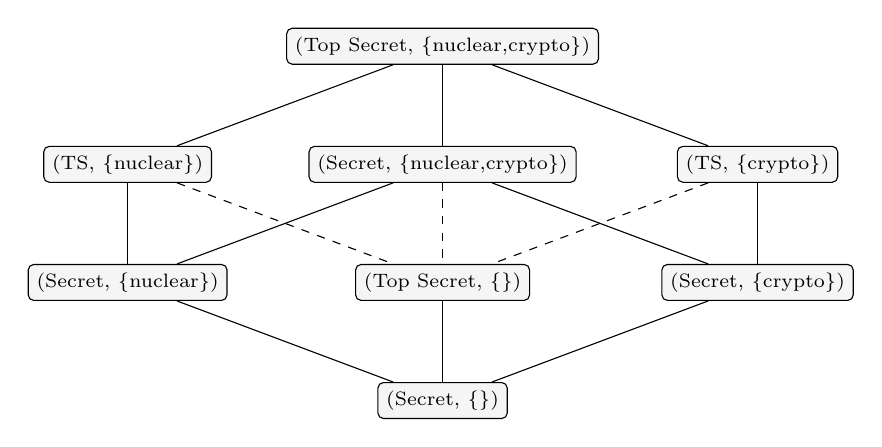
\begin{tikzpicture}[font=\scriptsize,
  c/.style={draw,rounded corners=2pt,fill=gray!8,inner sep=3pt}]
  \node[c] (top) at (0,3) {(Top Secret, \{nuclear,crypto\})};
  \node[c] (tn)  at (-4,1.5) {(TS, \{nuclear\})};
  \node[c] (sc)  at (0,1.5) {(Secret, \{nuclear,crypto\})};
  \node[c] (tc)  at (4,1.5) {(TS, \{crypto\})};
  \node[c] (sn)  at (-4,0) {(Secret, \{nuclear\})};
  \node[c] (ts0) at (0,0) {(Top Secret, \{\})};
  \node[c] (scr) at (4,0) {(Secret, \{crypto\})};
  \node[c] (bot) at (0,-1.5) {(Secret, \{\})};
  % aristas de dominancia (el de arriba domina al de abajo)
  \draw (top)--(tn); \draw (top)--(sc); \draw (top)--(tc);
  \draw (tn)--(sn); \draw[dashed] (tn)--(ts0);
  \draw (sc)--(sn); \draw (sc)--(scr); \draw[dashed] (sc)--(ts0);
  \draw (tc)--(scr); \draw[dashed] (tc)--(ts0);
  \draw (sn)--(bot); \draw (ts0)--(bot); \draw (scr)--(bot);
\end{tikzpicture}
\end{center}
\diagcaption{Retículo (diagrama de Hasse) del libro: cada arista sube hacia el que \textbf{domina}. (Secret,\{nuclear\}) y (Secret,\{crypto\}) \textbf{no son comparables} (ninguna lista de etiquetas contiene a la otra) $\Rightarrow$ están separados.}

A nivel implementación es simple: a cada objeto y a cada sujeto se le almacena como metadata un nivel y una lista de etiquetas; resolver cada operación con las dos reglas es directo.

\begin{ojo}
El error más penalizado de la unidad: \textbf{confundir las direcciones de lectura/escritura}. BLP (confidencialidad) es \textbf{read down / write up}; Biba (integridad) es lo opuesto. No alcanza con saber ``arriba/abajo'': hay que decir bien si es confidencialidad o integridad.
\end{ojo}

%======================================================================
\subsection{Modelos de Integridad: Biba y Clark-Wilson}
%======================================================================

\subsubsection{Modelo Biba}

Creado por Kenneth J.\ Biba. Fue el primer modelo público que \textbf{no buscaba confidencialidad sino proteger la integridad}. Es en realidad una familia de $\sim 7$ modelos. Define \textbf{niveles de integridad} (calidad/confiabilidad de la información). Una clasificación alternativa que el profesor prefiere: \emph{información no confiable, poco confiable, confiable, muy confiable, fidedigna}. Importante en sistemas documentales / de evidencia: contabilidad histórica, registros financieros que hay que retener, sistemas judiciales, medios de prensa, declaraciones fiscales.

\paragraph{Biba estricto.} Es Bell-LaPadula \textbf{al revés}:
\begin{definicion}{Reglas de Biba estricto}
\textbf{Lectura}: un sujeto puede leer un objeto si y solo si el nivel de integridad del \textbf{objeto} es igual o superior al del sujeto $\Rightarrow$ \textbf{``no read down''}.\\
\textbf{Escritura}: un sujeto puede escribir un objeto si y solo si el nivel de integridad del \textbf{objeto} es igual o menor al del sujeto $\Rightarrow$ \textbf{``no write up''}.
\end{definicion}

\begin{center}
\textbf{Biba (integridad): READ UP, WRITE DOWN.} (Invertir las flechas de un retículo BLP da Biba.)
\end{center}

\begin{center}
\begin{tikzpicture}[font=\scriptsize,
  lvl/.style={draw,rounded corners=3pt,minimum width=1.9cm,minimum height=0.6cm},
  ok/.style={-{Stealth},green!55!black,thick},
  no/.style={-{Stealth},red!75!black,thick,dashed}]
  % ---- BLP (izquierda) ----
  \node[font=\bfseries\footnotesize] at (0,3.6) {BLP (confidencialidad)};
  \node[lvl,fill=red!25]    (bh) at (0,2.6) {alto};
  \node[lvl,fill=orange!30] (bm) at (0,1.5) {medio (S)};
  \node[lvl,fill=green!25]  (bl) at (0,0.4) {bajo};
  \node[circle,fill=blue!20,draw,minimum size=0.42cm] (bs) at (2.0,1.5) {S};
  \draw[ok] (bs) to[bend right=12] (bl.east);   % read down
  \draw[no] (bs) to[bend left=12]  (bh.east);    % no read up
  \draw[ok] (bs) to[bend left=28]  (bh.east);    % write up
  \node[green!45!black] at (2.7,0.5) {read};
  \node[green!45!black] at (2.7,2.6) {write};
  % ---- Biba (derecha): retículo invertido ----
  \node[font=\bfseries\footnotesize] at (6,3.6) {Biba (integridad)};
  \node[lvl,fill=red!25]    (ih) at (6,2.6) {alto};
  \node[lvl,fill=orange!30] (im) at (6,1.5) {medio (S)};
  \node[lvl,fill=green!25]  (il) at (6,0.4) {bajo};
  \node[circle,fill=blue!20,draw,minimum size=0.42cm] (is) at (8.0,1.5) {S};
  \draw[ok] (is) to[bend left=12]  (ih.east);    % read up
  \draw[no] (is) to[bend right=12] (il.east);    % no read down
  \draw[ok] (is) to[bend right=28] (il.east);    % write down
  \node[green!45!black] at (8.7,2.6) {read};
  \node[green!45!black] at (8.7,0.5) {write};
\end{tikzpicture}
\end{center}
\diagcaption{Biba es el \textbf{espejo} de BLP: las flechas de lectura y escritura están invertidas. Confidencialidad lee abajo / escribe arriba; integridad lee arriba / escribe abajo.}

Intuición: ``uno es tan confiable como las fuentes que utiliza''. Para considerar a un sujeto confiable, la información en la que se basa debe ser de igual o mayor confianza (no puede leer información dudosa). Y lo que un sujeto genera/escribe tiene a lo sumo su mismo nivel, nunca mayor. Ejemplo: el SO te advierte al ejecutar un archivo bajado de Internet (origen poco confiable) y no si lo bajaste del App Store.

\paragraph{Biba Low-Watermark.} Variante \textbf{dinámica} (vs.\ las estáticas). No restringe la lectura: cualquier sujeto puede leer cualquier objeto, pero al hacerlo \textbf{el nivel de integridad del sujeto se reclasifica al mínimo} entre el que tenía y el del objeto. Si interactúa con algo de baja integridad, su nivel baja automáticamente, y deberá revalidarse para recuperar el nivel anterior. Base de muchos sistemas ``adaptativos''.

\begin{examen}
Biba Low-Watermark fue tomado en el Recuperatorio 2025. Recordá: \emph{lectura libre, pero el sujeto baja su nivel al del objeto leído (toma el mínimo)}.
\end{examen}

\subsubsection{Modelo Clark-Wilson}

Creado por David D.\ Clark y David R.\ Wilson. Modelo de \textbf{integridad} más acotado, pero introduce conceptos clave. Opera en un escenario con información y sujetos confiables y no confiables al mismo tiempo:
\begin{itemize}[nosep]
  \item Si sujeto e información son no confiables, que hagan lo que quieran.
  \item Un sujeto confiable no puede usar información no confiable; información confiable no puede ser usada por un sujeto no confiable.
\end{itemize}

¿Qué pasa cuando un sujeto confiable quiere usar información no confiable? Entra el mecanismo:
\begin{itemize}[nosep]
  \item Los datos pueden ser \textbf{restringidos/protegidos (CDI, Constrained Data Item)} o \textbf{sin restricción (UDI, Unconstrained Data Item)}.
  \item Los datos restringidos solo se modifican mediante un \textbf{Proceso de Transformación (TP)}.
  \item Hay un \textbf{Proceso de Verificación de Integridad (IVP)} independiente que valida.
  \item \textbf{Separation of duty (separación de tareas/privilegios)}: quien modifica los datos no puede ser el mismo que verifica la integridad.
\end{itemize}

Reglas de certificación y enforcement (del modelo formal): C1 IVP valida estado de CDI; C2 los TP preservan estado válido; C3 separación de tareas adecuada; C4 los TP escriben a log; C5 los TP validan los UDI. E1 los CDI se cambian solo por TP autorizados; E2 usuarios autorizados para TP; E3 usuarios autenticados; E4 las listas de autorización las cambia solo el security officer.

\begin{destacado}
\prof{La idea de este modelo de arbitración de Clark-Wilson es la base por la cual existen los kernels del sistema operativo y existe el concepto de User Space / Kernel Space como cosas separadas.}
Ejemplo bancario: para mover montos altos hacen falta dos personas (o procesos independientes), una verifica las firmas y otra ejecuta la transacción. En el SO, un \emph{syscall} arma datos en user space, un proceso los transforma/mueve a kernel space, otro proceso verifica su integridad y recién ahí se ejecuta en el espacio protegido.
\end{destacado}

\subsubsection{Más allá de los modelos teóricos}

Son modelos teóricos, difíciles de aplicar enteros a un sistema. No esperes encontrar el nombre explícito, pero aparecen partes:
\begin{itemize}[nosep]
  \item Compartimentos de BLP $\rightarrow$ sistemas que manejan \textbf{información médica} (regulatorios).
  \item Biba $\rightarrow$ sistemas de clasificación y archivo para \textbf{medios de prensa, legajos judiciales, declaraciones fiscales}.
  \item Clark-Wilson $\rightarrow$ concepto \textbf{kernel space / user space}.
\end{itemize}

%======================================================================
\subsection{Control de Acceso: clasificación}
%======================================================================

\begin{definicion}{Control de acceso}
Mecanismo de seguridad que regula quién puede acceder a qué recursos de la aplicación y bajo qué condiciones.
\end{definicion}

Dos grandes familias:

\begin{definicion}{Mandatory Access Control (MAC)}
Control que se aplica en forma \textbf{obligatoria} a todos los accesos de los sujetos a los objetos. Existen reglas universales que se aplican a todos. Los modelos vistos (BLP, Biba) son MAC. Se aplica sobre: todos los accesos, los cambios en las reglas/atributos, y el intercambio de información entre sujetos.
\end{definicion}

\begin{definicion}{Discretionary Access Control (DAC)}
La asignación y modificación de permisos queda a \textbf{discreción} del sujeto responsable del objeto o de un administrador. Las propiedades de seguridad las da el administrador según cómo configure, no el sistema. Típico de repositorios donde los sujetos crean los objetos (file systems, object storage).
\end{definicion}

MAC es muy rígido; para sistemas de propósito general (SO, bases de datos, suites de oficina) los controles tienden a ser \textbf{discrecionales} por flexibilidad.

\subsubsection{Control discrecional por extensión}

Definir el conjunto de accesos \emph{enumerándolos} uno por uno.

\paragraph{Matriz de acceso.} Matriz centralizada: sujetos (filas) $\times$ objetos (columnas); en cada celda, las acciones permitidas para esa combinación. Simple de entender, pero con problemas: escalabilidad (crece violentamente), eficiencia de búsqueda, mantenimiento propenso a errores, espacio, y mala adaptación a entornos dinámicos. Para una computadora una matriz enorme no es problema; \textbf{el cuello de botella es el humano} que debe cargar los valores a discreción.

\begin{ojo}
Falso clásico de parcial: \textbf{``una matriz de acceso bien diseñada evita el flujo de información no deseado''}. \textbf{FALSO}. La matriz (DAC, por extensión) solo controla el acceso \emph{directo}; no garantiza control de flujo de información. Para eso hacen falta modelos MAC tipo Bell-LaPadula (la *-property es justamente lo que controla el flujo).
\end{ojo}

\begin{center}
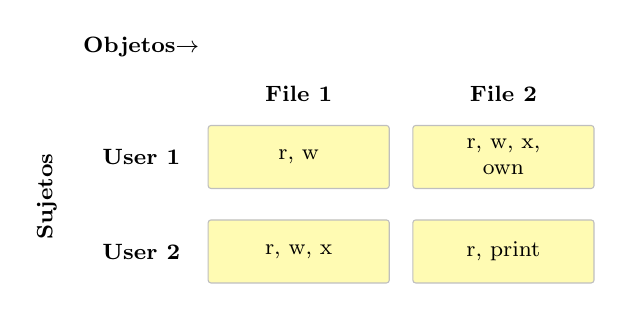
\begin{tikzpicture}[font=\footnotesize,
  obj/.style={font=\footnotesize\bfseries},
  perm/.style={fill=yellow!30,draw=gray!50,rounded corners=1pt,minimum width=2.3cm,minimum height=0.8cm,align=center}]
  % cabeceras de objetos
  \node[obj] at (2.0,1.0) {File 1};
  \node[obj] at (4.6,1.0) {File 2};
  \node[obj] at (0,1.6) {\textsc{Objetos}$\rightarrow$};
  \node[obj,rotate=90] at (-1.2,-0.3) {\textsc{Sujetos}};
  % filas
  \node[obj] at (0,0.2) {User 1};
  \node[obj] at (0,-1.0) {User 2};
  \node[perm] at (2.0,0.2) {r, w};
  \node[perm] at (4.6,0.2) {r, w, x,\\ own};
  \node[perm] at (2.0,-1.0) {r, w, x};
  \node[perm] at (4.6,-1.0) {r, print};
\end{tikzpicture}
\end{center}
\diagcaption{Matriz de acceso: sujetos (filas) $\times$ objetos (columnas); cada celda lista las acciones permitidas (basado en la slide ``Control por extensión'').}

\begin{center}
\begin{tikzpicture}[font=\scriptsize,
  box/.style={draw=gray!60,rounded corners=2pt,minimum height=0.65cm,inner sep=4pt}]
  % ACL: por columna (objeto)
  \node[font=\footnotesize\bfseries] at (1.6,2.2) {ACL (por columna $=$ objeto)};
  \node[box,fill=blue!8] (f1) at (0,1.4) {File 1};
  \node[box,fill=yellow!25,right=0.3 of f1] (f1a) {User1: r,w};
  \node[box,fill=yellow!25,right=0.2 of f1a] (f1b) {User2: r,w,x};
  \node[box,fill=blue!8] (f2) at (0,0.4) {File 2};
  \node[box,fill=yellow!25,right=0.3 of f2] (f2a) {User1: r,w,x,own};
  \node[box,fill=yellow!25,right=0.2 of f2a] (f2b) {User2: r,print};
  \draw[-{Stealth}] (f1) -- (f1a); \draw[-{Stealth}] (f1a) -- (f1b);
  \draw[-{Stealth}] (f2) -- (f2a); \draw[-{Stealth}] (f2a) -- (f2b);
  % Capabilities: por fila (sujeto)
  \node[font=\footnotesize\bfseries] at (1.6,-0.6) {Capabilities (por fila $=$ sujeto)};
  \node[box,fill=red!8] (u1) at (0,-1.4) {User 1};
  \node[box,fill=green!18,right=0.3 of u1] (u1a) {File1: r,w};
  \node[box,fill=green!18,right=0.2 of u1a] (u1b) {File2: r,w,x,own};
  \node[box,fill=red!8] (u2) at (0,-2.4) {User 2};
  \node[box,fill=green!18,right=0.3 of u2] (u2a) {File1: r,w,x};
  \node[box,fill=green!18,right=0.2 of u2a] (u2b) {File2: r,print};
  \draw[-{Stealth}] (u1) -- (u1a); \draw[-{Stealth}] (u1a) -- (u1b);
  \draw[-{Stealth}] (u2) -- (u2a); \draw[-{Stealth}] (u2a) -- (u2b);
\end{tikzpicture}
\end{center}
\diagcaption{Descomposición de la matriz: \textbf{ACL} recorre por columnas (a cada objeto, quién puede); \textbf{Capabilities} recorre por filas (a cada sujeto, a qué puede). Misma información, distinta forma de almacenarla.}

\paragraph{ACL (Access Control List).} Como las matrices reales son \textbf{dispersas} (permisos por ``islas''), se representan de forma compacta: para cada objeto, la lista de pares (sujeto, acción) permitidos. Es la misma información que la matriz, pero compacta. Se complementa con \textbf{permisos por defecto}, \textbf{grupos/agrupaciones} y \textbf{patrones} (\texttt{/users/*}, \texttt{/home/**/*.tmp}).

\subsubsection{Control discrecional por comprensión}

Definir el conjunto de accesos por sus \textbf{propiedades}, mediante \textbf{reglas} más compactas que reconstruyen la matriz bajo demanda. Tres modelos según criterio de agrupación:
\begin{itemize}[nosep]
  \item \textbf{RBAC (por roles)}: se estereotipan \textbf{roles} (Account Manager, DBA, Gestor de pacientes, Analista de compras\dots) que agrupan permisos; los roles se asignan a sujetos o grupos. Tras definir los roles, la gestión diaria es simple. (En sistemas tradicionales un usuario tiene un solo rol; en los complejos puede tener varios, lo que genera conflictos.) Algunos libros lo llaman MAC; en realidad la asignación de roles suele ser discrecional.
  \item \textbf{ABAC (por atributos)}.
  \item \textbf{RuBAC (por reglas)}: no asigna sujetos como los roles; usa una \textbf{lista ordenada de reglas} (Principal, Objeto, Tipo de Acceso, Permitido/Bloqueado) y aplica una política de resolución.
\end{itemize}

\begin{ojo}
Para usuarios \textbf{anónimos} conviene \textbf{ACL sobre Capabilities (CAP)} (parcial 2018). Las capabilities asocian permisos al sujeto (necesita identidad/token); con usuarios anónimos no hay a quién asociar la capability, así que conviene listar en el objeto quién puede (ACL).
\end{ojo}

%======================================================================
\subsection{Resolución de conflictos entre reglas}
%======================================================================

Cuando varias reglas aplican de forma contradictoria (o cuando se combinan varios mecanismos de control sobre la misma interacción), hay que resolver el conflicto. Es \textbf{crucial} entender cómo resuelve cada sistema, porque \emph{el mismo juego de reglas da resultados distintos según la política de resolución}.

\begin{itemize}[nosep]
  \item \textbf{First match}: las reglas tienen orden; se aplica la \textbf{primera} que hace match.
  \item \textbf{Best match}: aplica la regla \textbf{más específica} (antes que las generales).
  \item \textbf{Deny over Allow}: cualquier regla que deniegue explícitamente tiene precedencia sobre las que permiten (equivale a: si hay múltiples reglas que aplican, \emph{todas} deben permitir; si no, se deniega).
  \item \textbf{Grant-all / augment / override}: políticas adicionales (grant-all $\approx$ permitir si alguna regla permite).
\end{itemize}

\paragraph{Ejemplo (firewall).} Reglas ordenadas; conexión $10.1.1.1 \Rightarrow 20.1.1.1{:}80$. Matchean la regla específica (\texttt{10.1.1.1 \dots Accept}) y la general (\texttt{10.1.1.0/24 \dots Deny}).
\begin{itemize}[nosep]
  \item \textbf{First match}: gana la primera $\Rightarrow$ \textbf{Accept}.
  \item \textbf{Best match}: gana la más específica $\Rightarrow$ depende del caso (para $10.3.3.9 \Rightarrow 20.3.3.9{:}80$, la específica \texttt{Deny} gana sobre \texttt{10.3.3.0/24 Accept}).
  \item \textbf{Deny over Allow}: como hay una regla que deniega, \textbf{se frena} $\Rightarrow$ Deny.
\end{itemize}
En first-match las reglas dicen ``no permitas esta red salvo desde tal servidor''; en best-match ``permití toda la red salvo tal IP''. La forma de escribir las reglas cambia según el motor.

\begin{examen}
\textbf{Ejercicio recurrente (2015, 2016, Recup 2023):} dado $\mathrm{ACL}(o)=\{(\text{Manuel},r),(\text{Directivos},w),(*,w)\}$, donde Manuel \emph{es} Directivo, decidir bajo qué política puede \textbf{leer} y \textbf{escribir}.
\begin{itemize}[nosep]
  \item \textbf{Leer ($r$)}: solo la regla $(\text{Manuel},r)$ otorga lectura. Manuel \textbf{puede leer} bajo cualquier política que considere esa regla (first-rule si está primero, grant-all, augment).
  \item \textbf{Escribir ($w$)}: las reglas $(\text{Directivos},w)$ y $(*,w)$ otorgan escritura y Manuel encaja en ambas; ninguna regla la deniega, así que \textbf{puede escribir}.
  \item Bajo \textbf{grant-all}: alcanza con que una regla lo permita $\Rightarrow$ Manuel puede leer Y escribir.
  \item Razonar siempre: qué reglas matchean al sujeto, qué accede cada una, y cómo combina la política elegida (first-rule, grant-all, override, augment).
\end{itemize}
\end{examen}

\subsubsection{Reglas basadas en contexto}

El \textbf{contexto} son los datos asociados al sujeto, objeto, momento o lugar del acceso, que cambian independientemente de las reglas: momento del día, ubicación geográfica del origen, departamento del que accede, si el usuario estaba de vacaciones, nivel de confiabilidad de la máquina. Permiten detectar anomalías:
\begin{itemize}[nosep]
  \item Login desde China y desde Argentina con $5$ min de diferencia.
  \item Usuaria de licencia por maternidad que se loguea a una base de datos sensible.
  \item Usuario que abre dos VPN en menos de $5$ min con dos IP distintas.
\end{itemize}
Su nicho son los \textbf{sistemas de prevención de fraude}. (Un fraude es un abuso \emph{dentro} de las reglas del sistema; un problema de seguridad es un abuso \emph{salteándose} las reglas.) Son complejos; en el modelo \textbf{Zero-Trust} se define una entidad externa (\textbf{Policy Engine}) que evalúa todas las condiciones de contexto.

\subsubsection{Open Policy Agent (OPA)}

Framework estándar que unifica, mediante un lenguaje programable, la implementación de políticas de decisión, \textbf{desacoplando} la política del sistema de control. El servicio delega cada decisión a OPA: le envía una \emph{query} (JSON) y recibe una \emph{decision} (JSON). OPA evalúa una \textbf{política (Rego)} contra \textbf{datos contextuales (JSON)}. Las políticas se escriben en el lenguaje \textbf{Rego} (ej.\ en Kubernetes, denegar despliegues de imágenes que no vengan de un dominio dado).

%======================================================================
\subsection{Ejemplos reales de control de acceso}
%======================================================================

\begin{itemize}[nosep]
  \item \textbf{Unix/Linux file system}: ``engañosamente simple''. Permisos \texttt{rwx} en 3 secciones (usuario / grupo / otros). Tipo de archivo: \texttt{d} directorio, \texttt{-} archivo regular, \texttt{l} symlink. Al crear, un archivo hereda atributos del directorio; \texttt{umask} define una máscara que quita permisos a los archivos nuevos. Es \textbf{DAC}.
  \item \textbf{SELinux} (Security Enhanced): control \textbf{adicional al DAC}, basado en reglas que responden ``¿puede este sujeto acceder a este objeto?''. Procesos y recursos tienen un \emph{SELinux context} (ej.\ \texttt{/var/tmp: t\_var\_tmp}, Port 80: \texttt{t\_port\_www}). Usa macros que expanden a conjuntos de reglas. Permite que dos procesos con UID 0 (root) tengan restringido el acceso a los recursos del otro. Se usa en \emph{hardening} de servidores.
  \item \textbf{Windows file system}: DAC con dueño; usuarios y grupos; nivel básico y avanzado (más granular, $\sim 11$--$13$ operaciones). \textbf{Herencia} de permisos del contenedor, que \emph{persiste a la creación} (a diferencia de Unix). Calcula \textbf{permisos efectivos}; \textbf{Deny tiene precedencia sobre Allow}; reglas locales sobre heredadas. Cada entrada puede Allow / Deny / dejar en blanco (en blanco $=$ respeta el heredado).
  \item \textbf{PostgreSQL}: modelo basado en \textbf{roles} (un rol $=$ usuario, grupo u otro rol; propiedad \texttt{LOGIN}). Todo objeto creado por un rol tiene a ese rol como \textbf{owner} (DAC). \textbf{Policies} (Row Level Security) permiten need-to-know a nivel de registros (ej.\ cada vendedor ve solo sus clientes vía \texttt{salesperson\_id = current\_user}).
  \item \textbf{Squid Web Proxy}: proxy web que controla por dónde navegan los usuarios. Sistema de reglas (mal llamado ACL) de tipo \textbf{MAC}; reglas ordenadas que filtran por dominio, protocolo, URL, headers, \textbf{listas negras (blacklists)}. En la facultad bloquea sitios de streaming con esta tecnología.
  \item \textbf{AWS}: combina dos mecanismos: \textbf{policies asociadas al Principal (MAC)} (definidas para la cuenta, por administradores) y \textbf{policies asociadas al Recurso (DAC)} (las define quien crea el recurso, ej.\ S3 bucket policy).
  \item \textbf{API Gateway}: capa delante de las APIs; control basado en reglas (MAC) por URL, dominio, headers, method; y por contexto (req/seg máximos, ancho de banda).
\end{itemize}

\subsubsection{OAuth 2.0 (Open Authorization)}

Estándar de \textbf{autorización} para que aplicaciones accedan a recursos en nombre del usuario \textbf{sin compartir sus credenciales}. Funciona emitiendo \textbf{tokens de acceso temporales y específicos}. Es el ``entrar con tu cuenta de Google''.

Flujo: el usuario (Resource Owner) accede a la aplicación; la app lo redirige al \textbf{Authorization Server}, que lo autentica y le muestra la pantalla de consentimiento; al aceptar, el servidor envía un \textbf{authorization code} a la app, que lo intercambia por un \textbf{access token}; con ese token la app pide el recurso al \textbf{Resource Server}.

\begin{itemize}[nosep]
  \item \textbf{Access token} (vida corta: una hora, días) + \textbf{refresh token} (uso único; al usarlo devuelve un access y un refresh nuevos). Mecanismo para recuperarse ante robo de tokens y sostener la ``sesión infinita''.
  \item \textbf{Scope (DAC)}: permisos específicos que la app solicita (ver email, postear, leer calendario\dots). Se muestran en la pantalla de consentimiento; el token se limita a los scopes otorgados. Cada servicio verifica que el token sea válido y contenga su scope. Quien determina el control de acceso es \textbf{el dueño del recurso}.
\end{itemize}

%======================================================================
\subsection{Metodología: diseño de compartimentos (ejercicio estrella)}
%======================================================================

\begin{examen}
Es \textbf{el} ejercicio: dados sujetos, objetos y requisitos en \textbf{lenguaje natural}, construir un retículo de compartimentos. Casos históricos:
\begin{itemize}[nosep]
  \item \textbf{Confidencialidad}: restaurante Michelin (parciales 2015 y 2016) $\Rightarrow$ Bell-LaPadula.
  \item \textbf{Integridad}: clínica de cirugías estéticas (2013) y caso deepfake $\Rightarrow$ Biba.
\end{itemize}
\textbf{SIEMPRE hay que justificar requisito por requisito} y \textbf{nombrar bien la política}.
\end{examen}

\paragraph{Pasos.}
\begin{enumerate}[nosep]
  \item \textbf{Identificar el objetivo de seguridad}: ¿el enunciado pide \emph{ocultar} información (confidencialidad $\Rightarrow$ BLP) o \emph{proteger la calidad/origen} de la información (integridad $\Rightarrow$ Biba / Clark-Wilson)? El deepfake/integridad: ``Necesitan estructurarse con un modelo similar a Biba''.
  \item \textbf{Listar sujetos y objetos} del enunciado.
  \item \textbf{Definir los niveles} (jerarquía vertical) y las \textbf{etiquetas/categorías} (need-to-know horizontal: áreas, proyectos, temas que deben ir separados).
  \item \textbf{Asignar a cada sujeto y objeto su compartimento} $(\text{nivel},\{\text{etiquetas}\})$, justificando con el requisito que lo motiva.
  \item \textbf{Dibujar el retículo} con la relación de dominancia (orden parcial): aristas hacia el que domina; compartimentos sin etiquetas comparables quedan separados.
  \item \textbf{Verificar cada requisito} contra las reglas del modelo (read down/write up para BLP; read up/write down para Biba), uno por uno.
  \item \textbf{Nombrar la política} explícitamente (BLP ``no read up, no write down'' / Biba ``no read down, no write up'').
\end{enumerate}

\begin{examen}
\textbf{Identificar la política dado un retículo} (parcial 2018, jerarquía CEO $\to$ Gerentes $\to$ Empleado):
\begin{itemize}[nosep]
  \item Mirar las flechas/dirección de los flujos permitidos. Si el flujo de \emph{lectura} va hacia abajo (un superior lee lo de abajo) y la \emph{escritura} hacia arriba $\Rightarrow$ \textbf{Bell-LaPadula} (confidencialidad).
  \item Si están \textbf{invertidas} (lectura hacia arriba, escritura hacia abajo) $\Rightarrow$ \textbf{Biba} (integridad). Invertir las flechas de un retículo BLP da Biba.
\end{itemize}
\end{examen}

\subsubsection{Chinese Wall / Muralla China}

Modelo de \textbf{conflicto de interés}. Se agrupan los objetos en \textbf{clases de conflicto de interés (COI / Conflict of Interest)}; dentro de cada clase hay \textbf{datasets de compañías (CD)}. La regla: un sujeto que accedió a datos de una compañía dentro de una clase de COI \textbf{no puede acceder a los datos de otra compañía competidora} de la misma clase (ya consultó a un competidor). Tomado en el parcial 2018.

\begin{center}
\begin{tikzpicture}[font=\footnotesize,
  coi/.style={draw,rounded corners=4pt,inner sep=8pt,dashed,thick},
  cd/.style={circle,draw,minimum size=1.1cm,inner sep=1pt,align=center}]
  % COI Bancos
  \node[cd,fill=blue!15]  (b1) at (0,0)   {Banco\\A};
  \node[cd,fill=blue!15]  (b2) at (1.8,0) {Banco\\B};
  \node[coi,fit=(b1)(b2),label={[font=\footnotesize\bfseries]above:COI Bancos}] {};
  % COI Petroleras
  \node[cd,fill=orange!20] (p1) at (5,0)   {Oil\\X};
  \node[cd,fill=orange!20] (p2) at (6.8,0) {Oil\\Y};
  \node[coi,fit=(p1)(p2),label={[font=\footnotesize\bfseries]above:COI Petroleras}] {};
  % sujeto
  \node[rectangle,draw,fill=green!15,rounded corners=2pt] (s) at (3.4,-2.4) {Consultor S};
  % accesos
  \draw[-{Stealth},green!55!black,thick] (s) -- (b1);
  \draw[-{Stealth},red!75!black,thick,dashed] (s) -- (b2);
  \draw[-{Stealth},green!55!black,thick] (s) -- (p1);
  \node[green!45!black,font=\scriptsize] at (-1.0,-1.45) {1.\ lee OK};
  \node[red!70!black,font=\scriptsize]   at (2.55,-1.45) {2.\ \textbf{bloqueado}};
  \node[green!45!black,font=\scriptsize] at (5.6,-1.2) {lee OK (otro COI)};
\end{tikzpicture}
\end{center}
\diagcaption{Chinese Wall: tras leer Banco A, el consultor \textbf{no puede} leer a Banco B (competidor del mismo COI), pero sí una petrolera de \emph{otro} COI.}

%======================================================================
\subsection{Mentalidad de seguridad (clase de consulta)}
%======================================================================

\begin{destacado}
De la clase de consulta, el profesor remarcó:
\begin{itemize}[nosep]
  \item Los ejercicios son \textbf{situaciones laborales} donde uno \emph{decanta} la política general a partir del enunciado.
  \item Hay que \textbf{``activar el chip paranoico''}.
  \item \textbf{Defensa en profundidad $=$ encadenar controles} (varias capas).
  \item Para el caso deepfake/integridad: \emph{``Necesitan estructurarse con un modelo similar a Biba''}.
\end{itemize}
\end{destacado}

\begin{examen}
\textbf{Ejercicio abierto tipo ``sos el CSO''}: pasos para responder.
\begin{enumerate}[nosep]
  \item \textbf{Identificar el objetivo de seguridad}: confidencialidad, integridad o disponibilidad (puede haber más de uno).
  \item \textbf{Elegir el modelo} acorde (BLP para confidencialidad; Biba/Clark-Wilson para integridad).
  \item \textbf{Definir la política} concreta (qué estados son seguros).
  \item \textbf{Bajar a reglas} (ACL, RuBAC, compartimentos, MAC/DAC, resolución de conflictos) y, si conviene, encadenar controles (defensa en profundidad).
\end{enumerate}
\end{examen}

\end{document}
